%!TEX root = /Users/domaubert/Documents/Lectures/cosmologie/cosmo_main.tex

\chapter{Formation des grandes structures}
\label{s:struct}
Les grandes structures de l'Univers\index{grandes structures} désignent de façon générique et tout à la fois la matière diffuse, les galaxies et amas de galaxies qui s'organisent sous l'effet de la gravitation. Aujourd'hui ces grandes structures produisent une distribution de matière 'filamentaire' où des surdensités côtoient des vides, reliées entre elles par des ponts de matériau. Elles résultent de l'action du mécanisme d'instabilité gravitationnelle\index{instabilité gravitationnelle} sur les faibles fluctuations de densité présentes dans l'Univers jeune et tracées par exemple par le CMB. Au cours des 13.8 milliards d'années, des surdensité de 0.001\% parviennent ainsi à croître pour atteindre des contrastes de densité mesurés d'au moins plusieurs centaines dans les galaxies aujourd'hui. Si un grande partie des processus à l'œuvre lors de la formation des grandes structures peuvent être saisis par une approche analytique, le problème ne peut être abordé dans toute sa complexité que via l'utilisation de simulations numériques, dites simulation cosmologiques.

\section{Densité et spectre de puissance}
L'un des objectifs de l'étude de la formation des grandes structures est de prédire comme la matière va s'organiser au cours de l'histoire de l'Univers. La quantité généralement suivie est le contraste de densité\index{contraste de densité} :
\begin{equation}
\delta(x,t) =\frac{\rho-\bar\rho}{\bar\rho}.
\end{equation}
En l'absence de création de masse et dans un Univers homogène et isotrope, la densité moyenne $\bar{\rho}$ est une quantité de référence constante dans l'espace et pour laquelle la variation temporelle est seulement due à la dilution cosmologique \sidenote{dont on rappelle qu'elle fait varier la densité en $a^{-3}$.}

Toutefois, le contraste de densité à une position $x$ donnée et à un instant donné $t$ est finalement porteur d'assez peu d'information cosmologique, puisque l'on cherche à obtenir des contraintes qui ont une valeur 'cosmologique', i.e. globales et génériques. La première étape vers un traitement cosmologique consiste à raisonner dans l'espace de Fourier\index{transformée de Fourier} et à considérer les \textit{modes} $\delta_k(t)$ d'une réalisation donnée de $\delta(x,t)$:
\begin{equation}
\delta(x,t)\sim\int_{k=-\infty}^\infty \delta_k(t) e^{ikx} dk
\label{e:fourdelta}
\end{equation}
L'équation \ref{e:fourdelta} représente la décomposition en série de Fourier du contraste de densité : en pratique cela revient à décomposer le champ de densité en une série de modes sinusoïdaux et dont les contributions des différentes fréquences sont données par $\delta_k$. En plus d'un intérêt mathématique, cette décomposition constitue une mise en pratique de 'cosmologisation' de la densité : on se met à suivre des modes sinusoïdaux délocalisés, de taille caractéristique $\lambda=2\pi/k$ et la position $x$ perd de l'importance en tant que telle. L'amplitude d'un mode $k$ est donné tout simplement par $|\delta_k|^2$: l'étude de cette amplitude et son éventuelle évolution temporelle nous renseigne globalement sur l'évolution des structures d'échelle caractéristique $\lambda$ au cours du temps et sur leurs contribution relatives. Cette amplitude est aussi appelée \textit{puissance} et l'ensemble des puissances de tous les modes $k$ est appelé \textit{spectre de puissance}\index{spectre de puissance}.

\paragraph{Champ aléatoire Gaussien} Le champ de matière cosmologique appartient semble-t-il à la classe des champs aléatoires gaussiens\index{champs aléatoire gaussien}. C'est une prédiction des théories inflationnaires et il semble observationnellement que ce soit le cas : in fine cela constitue une base de travail et éventuellement on pourra être amené à mesure des départs à cette gaussianité. Un champ aléatoire gaussien $\delta(\vec x)$ se caractérise par une densité de probabilité de type:
\begin{equation}
p(\delta(\vec x)) \sim \exp( -\delta (\vec x) C^{-1} \delta (\vec x)),
\end{equation}
où $C$ est une matrice de corrélation, généralement non diagonale. Cette matrice encode les corrélations qui peuvent apparaître dans le champ de matière : celui-ci possède généralement des structures possédant une certaine cohérence spatiale et cette dernière se manifeste en couplant le champ $\delta$ entre différentes positions via $C$ \sidenote{par exemple la structuration de la matière dans l'Univers est telle que les régions denses se trouvent plutôt à proximité d'autres régions denses.}. Une propriété intéressante est que la probabilité de la transformée de Fourier de $\delta (\vec x)$ suit le même type PDF:
\begin{equation}
p'(\delta_{\vec k})\sim \exp( -\delta_{\vec k}^* \tilde C^{-1} \delta_{\vec k}).
\end{equation}
Une propriété encore plus intéressante est que $\tilde C$ est diagonale si $\delta(\vec x)$ est un champ aléatoire gaussien: chaque mode de Fourier peut être suivi statistiquement indépendamment des autres. Par simple inspection, il apparaît que les composantes de cette matrice de corrélation sont les variances des modes:
\begin{equation}
\langle \delta_{\vec k}^* \delta_{\vec k'}\rangle = P(k)\delta_D(\vec k -\vec k')=\langle|\delta_{\vec k}|^2\rangle.
\end{equation}
Cette mesure de la variance ne dépend que la norme $k=|\vec k|$ du mode considéré (plusieurs modes partagent donc la même variance) et constitue le spectre de puissance $P(k)$ du champ de matière.

Cette quantité est destinée à être mesurée au cours du temps et nous renseigne sur la croissance des structures. Si certaines échelles bénéficient d'une croissance plus rapide que d'autres, cela se manifestera par une déformation du spectre de puissance aux échelles concernées.  Si le champ est vraiment un champ aléatoire gaussien, la connaissance de $P(k)$ suffit à complètement le définir : si des corrélations anisotropes sont détectées (dans les relevés de galaxies ou dans le CMB), elles confirmeront soit la nature non-gaussienne\index{non-gaussianité} des fluctuations primordiales soit l'existence de processus physiques qui génèrent de la non-gaussianité \sidenote{notons que le spectre de puissance ne permet pas de mesurer la non-gaussianité. Deux champs, l'un gaussien l'autre non, peuvent partager les mêmes variances. Il faut utiliser des statistiques d'ordres supérieurs pour pouvoir faire cette distinction.}.

Une quantité reliée au spectre de puissance est la fonction de corrélation à deux points\index{fonction de corrélation} $\xi (r)$: elle exprime l'excès de probabilité de trouver de la matière en deux points séparés d'une certaine distance $r$ par rapport à une distribution aléatoire. On peut démontrer que la fonction de corrélation à deux points est simplement la représentation du spectre de puissance dans l'espace des positions (donc sa transformée de Fourier):
\begin{equation}
\xi (r)\sim \int d\vec k P(k) e^{i k r}.
\end{equation}
Notons qu'à nouveau cette excès de probabilité de dépend que de la distance $r$ et non pas d'une orientation ou de positions spécifiques des 2 points considérés. Généralement, la fonction de corrélation à 2 points est utilisée si l'on a une description discrète du champ de densité: c'est le cas par exemple lorsque l'on utilise des galaxies comme traceurs de la matière dans les grands relevés. Si l'on travaille avec un champ continu (comme dans des travaux analytiques), on passe directement dans une représentation en mode de Fourier en utilisant le spectre de puissance $P(k)$: ce dernier présente l'avantage d'explicitement séparer les modes de tailles différentes, là où la fonction de corrélation à 2 points "mélange" les modes et peut donc être dominé par une échelle au détriment des autres, qui peuvent pourtant contenir une information pertinente.

\section{Longueur de Jeans}
Une quantité centrale dans l'étude de l'instabilité gravitationnelle est la longueur de Jeans\index{longueur de Jeans}, notée $\lambda_J$. Elle correspond à la longueur minimale  que doit avoir une structure pour s'effondrer sous l'effet de la gravitation. On y associe également une masse (la masse de Jeans\index{masse de Jeans}) $M_J$ donnée simplement par:
\begin{equation}
M_J=\frac{4\pi}{3}\bar\rho\lambda_J^3,
\end{equation}
,où $\bar \rho$ est la densité moyenne du milieu : une structure de masse supérieure à la masse de Jeans va s'effondrer. L'existence du grandeur critique pour que l'effondrement se réalise traduit l'existence d'une compétition entre la gravité et un autre processus que la gravité doit 'vaincre' pour que la structure collapse. En général cet autre processus est l'existence d'un support thermique qui fournit une pression à même de s'opposer à la gravitation. Pour du gaz, il s'agit généralement de la pression interne du gaz, pour des systèmes non-collisionnels (type gaz d'étoiles) c'est la dispersion de vitesse interne qui agit comme une barrière à l'effondrement.

L'expression de la longueur de Jeans peut s'obtenir avec un simple raisonnement: pour qu'une structure s'effondre il faut que l'information gravitationnelle se répartisse plus rapidement au sein d'une structure que l'information de support thermique. Dans un milieu de densité $\rho$ l'information gravitationnelle est transportée en un temps dynamique\index{temps!dynamique}
\begin{equation}
t_G\approx \frac{1}{\sqrt{G\rho}}.
\end{equation}
Pour un gaz la transmission de l'information de support thermique dépend de la vitesse du son\index{vitesse!du son} $c_s$ et de la taille de la structure $\lambda$:
\begin{equation}
t_p\approx\frac{\lambda}{c_s}.
\end{equation}
L'effondrement a lieu si $t_G<t_p$, donc si la taille de la structure considérée obéit à la condition:
\begin{equation}
\lambda >\frac{c_s}{\sqrt{G\rho}}\equiv \lambda_J.
\end{equation}
Faire baisser $\lambda_J$ revient à favoriser l'effondrement gravitationnel, le cas limite étant $\lambda_J \rightarrow 0$ où toute structure s'effondre. Ce régime s'obtient dans un milieu très dense ou bien très froid, i.e. sans support thermique.  A l'inverse, une grande valeur de $\lambda_J$ réduit la possibilité d'effondrement et $\lambda_J\rightarrow\infty$ revient à empêcher toute structure de s'effondrer: cela correspond à un milieu sous-dense, donc très léger, ou bien très chaud avec une grande vitesse du son. Pour un système non-collisionnel, la même expression existe pour la longueur de Jeans en remplaçant la vitesse du son par la dispersion de vitesse du milieu.

\subsection{Traitement perturbatif}
Une dérivation plus rigoureuse peut être obtenue par un traitement perturbatif au premier ordre. On considère un gaz de densité moyenne $\bar \rho$ et d'équation d'état:
\begin{equation}
\frac{dP}{d\rho}=c_s^2.
\end{equation}
Ce gaz obéit aux équation de Poisson\index{equation@équation!de Poisson}, qui est l'équation de champ de la gravité newtonienne:
\begin{equation}
\Delta \phi(x,t) = 4 \pi G \rho
\end{equation}
 et aux équations fluides, conservation de la masse\index{conservation de la masse}
 \begin{equation}
 \frac{\partial \rho}{\partial t} + \vec \nabla \rho \vec u=0,
 \end{equation}
 et conservation de l'impulsion\index{conservation de l'impulsion}
 \begin{equation}
 \frac{\partial \vec v}{\partial t} +\vec u \vec \nabla \vec u = -\frac{\vec \nabla P}{\rho}-\vec \nabla \phi.
 \end{equation}
 On réalise un traitement perturbatif (à 1D par simplicité)\sidenote{notons qu'on considère ici que le milieu n'est pas animé d'une vitesse globale à l'équilibre $v_0=0$ et que le milieu à l'équilibre ne présente pas de variations spatiales de potentiel : ce potentiel $\phi_0$ constant dans l'espace est sans influence dynamique et est donc ignoré}:
 \begin{eqnarray}
 \rho(x,t)&=&\bar \rho(1 +\delta(x,t))\\
 u(x,t)&=&v_1(x,t)\\
 \phi(x,t)&=&\phi_1(x,t)\\
 P&=&P_0+P_1(x,t)
 \end{eqnarray}
 En injectant ces développement, on parvient aisément à écrire:
 \begin{eqnarray}
 \frac{\partial \delta}{\partial t}&=&-\bar \rho \frac{\partial v_1}{\partial x}\\
 \frac{\partial}{\partial t}\frac{\partial v_1}{\partial x}+\frac{c_s^2}{\bar \rho}\frac{\partial^2 \delta}{\partial x^2}+\frac{\partial^2 \phi_1}{\partial x^2}&=&0
 \end{eqnarray}
 d'où l'équation maîtresse de l'instabilité:
 \begin{equation}
 \ddot \delta -c_s ^2\frac{\partial^2 \delta}{\partial x^2}=4\pi G \bar \rho \delta
 \end{equation}
 \subsection{Effondrement et Oscillations}
 Cette équation s'analyse plus facilement en prenant sa transformée de Fourier spatiale:
 \begin{equation}
 \ddot \delta_k +(c_s^2k ^2-4\pi G \bar \rho) \delta_k= 0.
 \end{equation}
 Deux régimes peuvent être facilement distingués:
 \begin{itemize}
 \item si $c_s^2 k^2> 4\pi G \bar \rho$ c'est une équation d'oscillateur harmonique. Le mode correspond à une onde sonore de pulsation $\omega=\sqrt{c_s^2 k^2-4\pi G \bar \rho}$. Cela correspond à des grandes fréquences spatiales, donc des petites structures: notons que leur fréquence temporelle est d'autant plus grande que ces structures sont petites.
 \item si $c_s^2 k^2< 4\pi G \bar \rho$, la solution est hyperbolique avec donc une contribution exponentielle croissante, qui correspond à l'instabilité gravitationnelle. Ce régime correspond aux faibles valeurs de $k$ donc aux grandes échelles. Le temps caractéristique d'instabilité est $\tau = (4\pi G \bar \rho - c_s^2k^2)^{-1/2}$ qui se résume au temps dynamique si k est suffisamment faible donc si le mode étudié est suffisamment grand. 
 \end{itemize}
 
 On remarque que le cas critique $\frac{4\pi^2c_s^2}{\lambda^2}=4\pi G \rho$ nous redonne la longueur de Jeans:
 \begin{equation}
 \lambda_J=c_s\sqrt{\frac{\pi}{G\rho}}
 \end{equation}
 
 \subsection{Cas cosmologique}
\newthought{Le cas cosmologique} se doit de prendre en compte l'expansion de l'Univers. Comme on le verra en fin de démonstration, cela change finalement peu de choses par rapport au cas exposé précédemment. Toutefois cette étude présente un intérêt technique en rapport avec la manipulation de grandeur comobiles dans des équations différentielles couplées. Pour cette raison le calcul sera décrit en détail.

\newthought{Les équations importantes} sont les mêmes que dans le cas d'un Univers statique\sidenote{$\rho$ est la densité de matière, $\vec u$ la vitesse, $\vec  r$ la position physique, $P$ la pression et $\phi$ le potentiel gravitationnel}:
\begin{eqnarray}
\frac{\partial \rho}{\partial t}+\frac{\partial \rho \vec u}{\partial \vec r}&=&0\\
\frac{\partial \vec u}{\partial t}+\vec u \cdot \frac{\partial \vec u}{\partial \vec r}&=&-\frac{1}{\rho}\frac{\partial P}{\partial \vec r}-\frac{\partial \phi}{\partial \vec r}\\
\frac{\partial^2 \phi}{\partial \vec r^2}&=&4\pi G \rho.
\end{eqnarray}
 La principale difficulté découle de la dépendance temporelle de la distance physique\index{distance!physique} $\vec r=a(t) \vec x(t)$ où $\vec x$ désigne la position comobile\index{distance!comobile} : la dérivée par rapport à $\vec r$ doit donc être prise avec précaution. Par commodité on préfère généralement écrire ces équations en fonction de données comobiles pour extraire au moins l'effet de flot cosmologique encodé par le facteur d'expansion $a(t)$.
 
La première étape consiste à transformer les dérivée temporelles prises à $\vec r$ constant en dérivée prises à $\vec x$ constant\sidenote{on rappelle que pour $f(r=a(t)x,t)$ alors $\left(\frac{\partial f}{\partial t}\right)_x=\left(\frac{\partial f}{\partial t}\right)_r+\frac{\partial f}{\partial \vec r}\frac{\partial \vec r}{\partial t}$}:
\begin{equation}
\left(\frac{\partial }{\partial t}\right)_r = \left(\frac{\partial }{\partial t}\right)_x-\frac{\dot a}{a}\vec x \cdot \left(\frac{\partial}{\partial \vec x}\right)_t,
\end{equation}
de même les dérivée spatiales deviennent:
\begin{equation}
\frac{\partial }{\partial \vec r}=\frac{1}{a}\frac{\partial}{\partial \vec x}.
\end{equation}
 Pour finir, il faut établir que la vitesse comporte une partie liée au flot de Hubble\index{Hubble!flot} \sidenote{ le terme $\dot a \vec x$ peut facilement se réecrire sous la forme $H \vec r$, i.e. la loi de Hubble}:
\begin{equation}
\dot {\vec u}=\dot a \vec x + a \dot {\vec x}= \dot a \vec x + \vec v
\end{equation}
 où $\vec v$ désigne une vitesse particulière superposée au flot cosmologique.
 Enfin la densité sera également exprimée en fonction de la densité de fond, $\bar \rho \sim a^{-3}$ qui subit l'expansion cosmologique :
 \begin{equation}
 \rho(\vec x,t) =\bar \rho(t)(1+\delta(\vec x,t)).
 \end{equation}
 
 \newthought{La conservation de la masse} est modifiée comme suit : nous allons prendre les différents termes un par un. La dérivée temporelle de la densité comprend 2 termes, le premier \sidenote{notez la dérivée temporelle de $\bar \rho\sim a^{-3}$ qui intervient ici }:
 \begin{eqnarray}
  \left(\frac{\partial \rho}{\partial t}\right)_x&=& \left(\frac{\partial \rho}{\partial t}\right)_r,\\
  &=&\bar \rho\frac{\partial \delta}{\partial t} -3\frac{\dot a}{a}\bar \rho (1+\delta),
 \end{eqnarray}
et le second:
\begin{eqnarray}
\frac{\dot a}{a}\vec x \cdot \frac{\partial \rho}{\partial \vec x}&=&\frac{\dot a }{a}\bar \rho \frac{\partial\delta}{\partial \vec x}.
\end{eqnarray}
Le terme de flux de cette même équation devient quant à lui:
\begin{eqnarray}
\frac{1}{a}\frac{\partial}{\partial \vec x}(\bar \rho(1+\delta)(\vec v + \dot a \vec x))&&\\
=\frac{\bar \rho}{a} \frac{\partial}{\partial \vec x}(\bar \rho(1+\delta)\vec v) + \frac{\bar \rho \dot a}{a} \frac{\partial}{\partial \vec x}(\bar \rho(1+\delta)\vec x)&&.
\end{eqnarray}
Le dernier terme de cette égalité peut être réecrit sous la forme:
\begin{eqnarray}
\frac{\bar \rho \dot a}{a} \frac{\partial}{\partial \vec x}(\bar \rho(1+\delta)\vec x)&&\\
=\bar \rho \frac{\dot a }{a} 3(1+\delta) +\bar \rho \frac{\dot a }{a} \vec x \cdot \frac{\partial \delta}{\partial \vec x}.
\end{eqnarray}
En rassemblant le tout on obtient l'équation de conservation de la masse dans sa formulation comobile:
\begin{equation}
\frac{\partial \delta}{\partial t}+\frac{1}{a}\frac{\partial}{\partial \vec x}((1+\delta)\vec v)=0
\end{equation}

 \newthought{L'équation d'Euler comobile} \index{equation@équation!d'Euler} se dérive de la même manière. Prenons le premier terme de dérivée temporelle de la vitesse:
 \begin{eqnarray}
 \left(\frac{\partial \vec u}{\partial t}\right)_r&=&\left(\frac{\partial \vec u}{\partial t}\right)_x-\frac{\dot a }{a}\vec x \cdot \frac{\partial \vec u}{\partial \vec x}.
\end{eqnarray}  
La dérivée temporelle à $\vec x$ constant donne:
\begin{eqnarray}
\left(\frac{\partial \vec u}{\partial t}\right)_x&=&\left(\frac{\partial \vec v}{\partial t}\right)_x + \ddot a {\vec x},
\end{eqnarray}
tandis que le terme de Hubble donne \sidenote{on utilise ${\vec e} \cdot \frac{\partial}{\partial \vec x}\vec x= \vec e$}:
\begin{eqnarray}
\frac{\dot a }{a}\vec x \cdot \frac{\partial \vec u}{\partial \vec x}&=&\frac{\dot a }{a}\vec x \cdot \frac{\partial \vec v}{\partial \vec x}+\frac{\dot a^2}{a}\vec x.
\end{eqnarray}
 Le terme d'advection ne présente pas de difficulté particulière \sidenote{on utilise ${\vec e} \cdot \frac{\partial}{\partial \vec x}\vec x= \vec e$} :
 \begin{eqnarray}
 \vec u \cdot \frac{\partial \vec u}{\partial \vec r}&=&\frac{1}{a}\vec v \cdot \frac{\partial \vec v}{\partial \vec x}+\frac{\dot a}{a}\vec x \cdot \frac{\partial \vec v}{\partial \vec x}\\
 &&+ \frac{\dot a^2}{a}\vec x +\frac{\dot a}{a}\vec v.
 \end{eqnarray}
 En rassemblant tous ces premiers termes on obtient une expression comobile pour le membre de gauche de l'équation d'Euler:
 \begin{equation}
 \left(\frac{\partial \vec v}{\partial t}\right)_x +\frac{\dot a}{a}\vec v+\frac{1}{a}\vec v \cdot \frac{\partial \vec v}{\partial \vec x} + \ddot a {\vec x}. 
 \label{e:geuler}
 \end{equation}
 Le terme correspondant aux forces de pressions\index{pression} de pose pas de difficulté tandis que le terme correspondant aux forces de gravitation peut être modifié en lui incluant le terme en $\ddot a {\vec x}$ de l'équation \ref{e:geuler}:
 \begin{eqnarray}
  \frac{\partial \phi}{\partial \vec r}&=&\frac{1}{a}(\frac{\partial \phi}{\partial \vec x}+a\ddot a \vec x)\\
  &=&\frac{1}{a}\frac{\partial \Phi}{\partial \vec x},
 \end{eqnarray}
 où $\Phi(\vec x,t)$ est un potentiel gravitationnel effectif, prenant en compte les effets de fonds changeant:
 \begin{equation}
 \Phi= \phi+\frac{a\ddot a {\vec x}^2}{2}.
 \end{equation}
En rassemblant partie différentielle et termes sources, on obtient une équation d'Euler comobile qui ressemble beaucoup à sa contrepartie physique avec l'inclusion d'un terme de friction de Hubble :
\begin{equation}
\left(\frac{\partial \vec v}{\partial t}\right)_x +\frac{\dot a}{a}\vec v+\frac{1}{a}\vec v \cdot \frac{\partial \vec v}{\partial \vec x}=-\frac{1}{a\bar \rho (1+\delta)}\frac{\partial P}{\partial \vec x}-\frac{1}{a}\frac{\partial \Phi}{\partial \vec x}.
\end{equation}

\newthought{L'équation de Poisson}\index{equation@équation!Poisson} doit également être reformulée en faisant notamment intervenir le potentiel effectif $\Phi$\sidenote{en utilisant $\frac{\partial^2}{\partial \vec x^2} {\vec x}^2=6$}:
\begin{eqnarray}
\Delta \phi &=&\frac{1}{a}\frac{\partial^2 \phi}{\partial \vec x^2}\\
&=&\frac{1}{a^2}\frac{\partial \Phi}{\partial \vec x^2}-3\frac{\ddot a}{a}\\
&=&4\pi G \bar \rho(1+\delta).
\end{eqnarray}
Or l'équation de Friedmann\index{equation@équation!Friedmann}\sidenote{$\frac{\ddot a}{a}=-\frac{4}{3}\pi G \bar \rho$} permet de relier l'évolution du facteur d'expansion avec la densité du fond et permet notamment d'établir que:
\begin{equation}
4\pi G \bar \rho a^2+3 a \ddot a=0,
\end{equation}
 d'où l'équation de Poisson comobile:
 \begin{equation}
 \frac{\partial^2 \Phi}{\partial \vec x^2}=4\pi G \bar \rho a^2 \delta
 \end{equation}
 
 \newthought{En présence d'expansion}, l'équation maîtresse devient (pour chaque mode de Fourier):
 \begin{equation}
  \ddot \delta_k +2H\dot \delta_k+ (\frac{c_s^2k ^2}{a^2}-4\pi G \bar \rho) \delta_k= 0.
  \label{e:epert}
 \end{equation}
 où toutes les quantités sont des quantités comobiles. On retrouve essentiellement la même équation et les mêmes conclusions s'imposent, à savoir instabilité si $\lambda >\lambda_J$ et oscillations sonores dans le cas inverse. On note toutefois la présence du terme $2H\dot \delta_k$ qui s'apparente à un terme d'amortissement dû à l'expansion. On montrera qu'à cause de ce terme qui tempère les solutions, les modes instables\index{modes instables} ne seront plus exponentiels mais en loi de puissance et les modes stables oscillants seront amortis sur des temps caractéristiques de l'ordre du temps de Hubble.
 
 A ce stade il faut rappeler, que le traitement décrit juste ici est approché. Par exemple la matière noire \sidenote{qui compose $80\%$ du bilan énergétique de la matière} ne peut pas, à priori, être correctement décrite par les équations 'fluides' utilisées ici. Comme ses particules sont non collisionelles, on ne peut réduire la pression\sidenote{qui est une mesure des propriétés du tenseur des dispersions de vitesses} à un scalaire et elle peut être anisotrope. La question se pose dans les même termes pour le rayonnement. Un traitement rigoureux doit passer par l'utilisation de l'équation de Boltzmann qui encode directement l'évolution de la fonction de distribution des ces fluides dans l'espace des phases et non celle des ses moments (densité, impulsion, etc...).  Heureusement le résultat obtenu reste très similaire à celui présenté dans l'équation \ref{e:epert} et elle fera donc l'affaire pour les raisonnements à suivre.
 
 L'autre difficulté est lié à la nature multi-fluide des perturbations. Nous avons:
 \begin{itemize}
 \item les photons: relativistes, avec une pression de rayonnement associée,
 \item les baryons: non-relativistes mais couplés avec le rayonnement avant la recombinaison. Les photons vont donc leur fournir une source de support dynamique bien plus importante que la simple pression thermique,
 \item la matière noire : non-relativiste et sans pression.
 \end{itemize}
 Ces 3 fluides vont évoluer selon des termes donnés par l'éq. \ref{e:epert}. Par ailleurs ces fluides sont couplés et s'influencent l'un l'autre : c'est vrai via la pression de rayonnement pour les baryons et les photons mais également via le terme $4\pi G \bar \rho \delta_k$. Ce terme trace une source gravitationnelle de perturbation et doit donc inclure toutes les contributions au bilan énergétique de l'Univers, photons compris. C'est notamment vrai durant les époques avant l'équivalence \sidenote{correspondant à $z>3000$ ou $t<80 000$ ans où matière et rayonnement contribuent de manière égale au bilan énergétique du cosmos} durant lesquelles la source principale de potentiel est la contribution des photons. En pratique, nous avons donc un jeu d'équations multiples couplées qu'on ne peut résoudre de façon analytique : les grands principes peuvent toutefois être explorés en appliquant des hypothèses raisonnables comme décrit dans les parties suivantes.
 
 \section{Croissance des perturbations : cas sub-horizon}
 \newthought{Les échelles explorées} dans cette partie sont suffisamment compactes pour être plus petites que l'horizon a un instant donné. Cela permet en particulier le transport d'une information dynamique au sein des structures en jeu, autorisant effondrement ou ondes de pression par exemple. L'équation à interpréter est celle donnée par l'eq. \ref{e:epert} et nous allons être amenés à distinguer 2 époques, avant l'équivalence (dominée par le rayonnement RD) et après l'équivalence (dominée par la matière MD). Les facteurs d'expansion et le paramètre de Hubble \sidenote{avec $H=\dot a/a$} durant RD sont donnés par :
 \begin{eqnarray}
 a&\sim& \sqrt{t},\\
 H&=&\frac{1}{2t},
 \end{eqnarray}
 tandis que les relations équivalentes durant MD sont données par:
 \begin{eqnarray}
 a&\sim&t^{2/3},\\
 H&=&\frac{2}{3t}.
 \end{eqnarray}
 
  \subsection{Matière sans pression}
Prenons d'abord le cas d'une matière sans pression, correspondant à celui de la matière noire : la vitesse du son est négligeable et pourra donc être annulée dans Eq. \ref{e:epert}.

\newthought{Durant l'époque dominée par le rayonnement}, le terme source de gravitation est dominé par la contribution des photons. Toutefois, on considèrera ce terme comme négligeable : les photons possèdent une pression intrinsèque élevée et une grande longueur de jeans. Ils ne peuvent se structurer et leur densité ne peut croître de façon substantielle \sidenote{de fait elle aura un comportement oscillant, voir section suivante}:
\begin{equation}
\bar \rho \delta_k \sim(\bar \rho \delta_k)_\gamma \sim 0.
\end{equation}
L'équation résultante pour la matière sans pression est donc: 
\begin{equation}
\ddot \delta_k+\frac{1}{t}\dot \delta \sim 0
\end{equation}
dont la solution est de type logarithmique:
\begin{equation}
\delta_{k,RD}\sim \log(t).
\end{equation}
Dans le cadre qui est le nôtre, une croissance logarithmique peut être assimiliée à une absence de croissance, au mieux à une croissance très lente.

\newthought{Durant l'époque dominée par la matière}, le terme source est dominé par la matière elle-même: toute croissance sera donc entretenue par une croissance du potentiel, conduisant naturellement à une augmentation de la perturbation. L'équation à traitée est donnée par:
\begin{equation}
\ddot \delta_k +2 H \dot \delta_k =4\pi G \bar\rho \delta_k.
\end{equation}
En introduisant explicitement les dépendances temporelles on obtient\sidenote{en utilisant $\bar \rho\sim\rho_c=\frac{3H^2}{8\pi G}$}:
\begin{equation}
\ddot \delta_k +\frac{4}{3t}\dot \delta_k - \frac{2}{3t^2}\delta_k=0.
\end{equation}
Cette équation possède une solution croissante donnée par \sidenote{il existe aussi une solution décroissante en $\delta=1/t$, qui est de peu d'intérêt car dominée par la solution croissante} :
\begin{equation}
\delta_{k,MD}\sim t^{2/3}\sim a(t).
\end{equation}
Le contraste avec la solution précédente est frappant: la présence d'un terme source de gravitation permet à la fluctuation de prospérer tandis que que son absence conduit à une non-augmentation de la perturbation.

\subsection{Matière avec pression}
Ce cas correspond à celui des baryons : durant ces époques pré-recombinaison, le couplage important entre les photons et les baryons confère à ces dernier une pression importante et une vitesse du son proche de la vitesse de la lumière $c_s\sim c$.

\newthought{Durant l'époque dominée par le rayonnement}, on continuera à négliger le terme source induit par les photons par contre le terme de pression ne peut plus être omis et l'équation des perturbations devient:
\begin{equation}
\ddot \delta_k+2H\dot \delta +c_s^2k^2 \delta \sim 0.
\end{equation}
La solution est oscillante avec un amortissement induit par l'expansion\sidenote{avec un temps caractéristique $\tau \sim{1/2H}$.}. De notre point de vue, c'est également une solution 'sous contrôle', non-croissante. En l'absence de gravitation, les fluctuations baryoniques s'organisent en ondes de pression.

\newthought{Durant l'époque dominée par la matière}, le terme source de gravitation devient non négligeable mais n'est pas dominé par les baryons\sidenote{qui ne représente que $20\%$ de la matière totale}. L'équation à résoudre devient alors \sidenote{ici $DM$ dénote la matière noire pour \textit{dark matter}.}:
\begin{equation}
\ddot \delta_k+2H\dot \delta +c_s^2k^2 \delta 4\pi G \bar\rho_{DM} \delta_{k,DM}
\end{equation}
On a donc un terme source de fond, mais ce terme n'est pas en mesure de produire une augmentation de l'amplitude des oscillations: ce terme évolue lentement par rapport aux temps caractéristiques d'oscillations et ne peut donc produire de résonances par exemple. Ce terme de forçage n'implique pas de croissance incontrôlée de l'amplitude des fluctuations baryoniques qui sont toujours dans un régime oscillant comme précédemment.

\newthought{Ces oscillations} constituent de notre point de vue une 'absence de croissance': les ondes de pressions passent mais ne 'grossissent pas'. En pratique c'est même l'opposé qui va se produire : à cause du couplage imparfait entre photons et rayonnement, la pression apportée par les photons ne garantit pas un entretien perpétuel des oscillations et elles vont s'amortir \sidenote{on parle aussi d'amortissement Silk\index{amortissement Silk}, du nom du physicien anglais à l'origine de la découverte de cet effet}. L'effet d'amortissement est même catastrophique au sens où toute structure baryonique contenant une masse inférieure à $10^{13} M_\odot$ \sidenote{et donc de taille inférieure à une certaine taille critique} doit être 'effacée' du spectre des fluctuations. Cette masse est supérieure à celle de la Voie Lactée actuellement : il faut donc trouver un mécanisme pour entretenir les fluctuations de masse inférieure à cette limite pour pouvoir expliquer les structures observées aujourd'hui.

\newthought{La matière noire}\index{matière noire} va fournir ce mécanisme: comme vu précédemment, la matière sans pression va voir ses fluctuations croître de façon permanente durant l'époque dominée par la matière. Au moment de la recombinaison, les baryons auront vu une grande partie de leurs fluctuations être amorties par l'amortissement que nous venons juste de mentionner. Toutefois la recombinaison s'accompagne de la perte de support de pression offert par le rayonnement \sidenote{permettant aux photons de s'échapper sous forme du rayonnement de fond diffus}: les baryons sont alors libres de s'effondrer dans les puits de potentiels crées par la matière noire. Vers un redshift $z\sim 100$ les fluctuations baryoniques ont convergé vers les fluctuations de la matière noire, autorisant la formation de structures de masses plus légères que la masse limite mentionnée précédemment.

\begin{figure}[htbp]
	\centering
		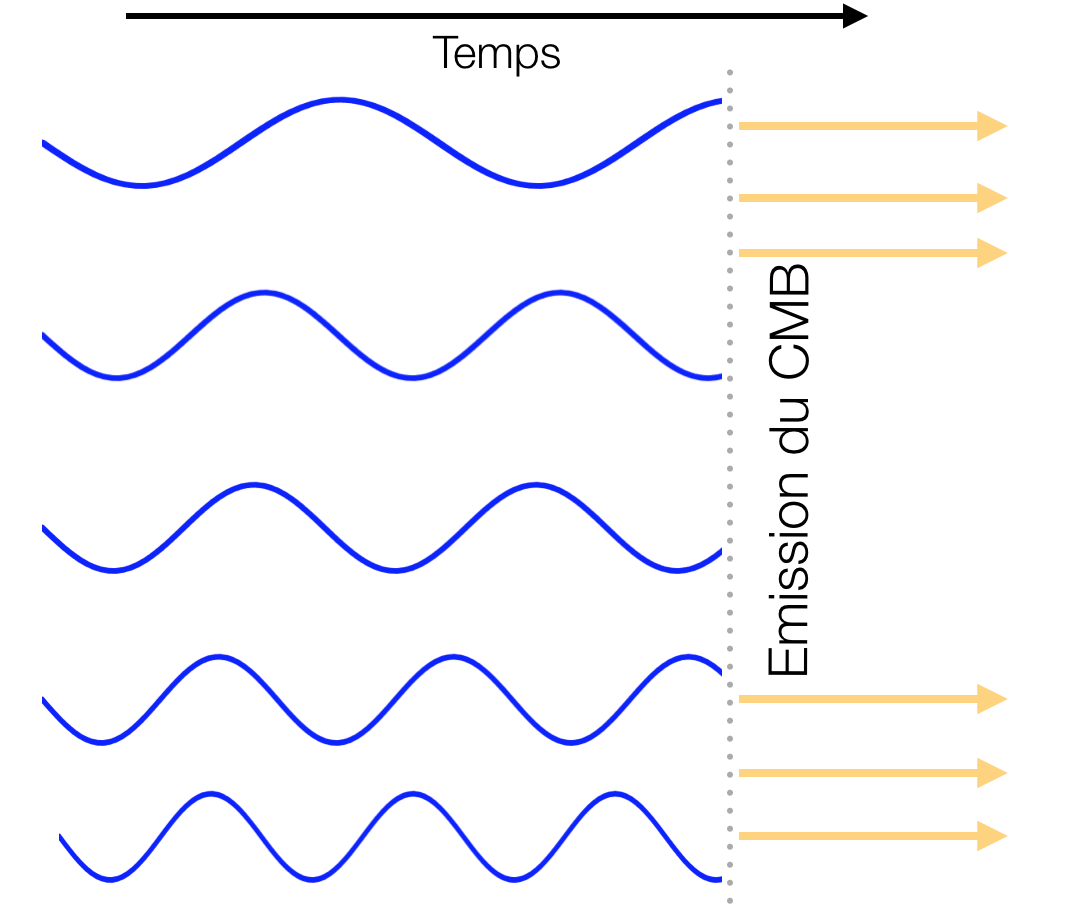
\includegraphics[height=12cm]{figs/bao1.png}
	\caption[Les oscillations baryoniques évoluent sur des fréquences différentes, dépendant de leur taille.]{Les oscillations baryoniques évoluent sur des fréquences différentes, dépendant de leur taille. Les grandes structures oscillent lentement, les petites rapidement. Certains modes vont être en extremum d'amplitude au moment de la recombinaison et donc au moment de la dernière diffusion du fond diffus cosmologique. Ces modes vont donc être privilégiés dans la carte du CMB.}
	\label{f:bao1}
\end{figure}


\newthought{Ces oscillations baryoniques}  sont des ondes accoustiques (BAOs, de l'anglais \textit{baryonic accoustic oscillations})\index{BAO} car elles sont entretenues par l'entrejeu entre gravité et pression (de rayonnement dans le cas présent). Par simple inspection de l'équation différentielle maîtresse, on peut constater que la fréquence d'oscillation dépend de la taille du mode étudié : un mode à grande fréquence spatiale implique une grande fréquence temporelle et vice-versa. Par conséquent, l'amplitude du mode au moment de la recombinaison va dépendre du mode en question : au moment de l'émission du fond diffus, certains modes seront en amplitude maximale, d'autres en amplitude plus modérée. En simplifiant (voir Fig. \ref{f:bao1}), on peut imaginer que certains modes vont osciller un nombre de fois exactement entier entre leur déclenchement et la recombinaison, parvenant ainsi à un extremum d'amplitude tandis que d'autres seront dans une phase quelconque avec des amplitudes moins remarquables. Les échelles qui se détachent sous la forme de 'pics' dans le spectre de puissance du fond diffus cosmologique (voir Fig. \ref{f:bao2}) sont la manifestation de ces modes qui parviennent en extremum d'amplitude au moment où le rayonnement fossile est produit.



\begin{figure}[htbp]
	\centering
		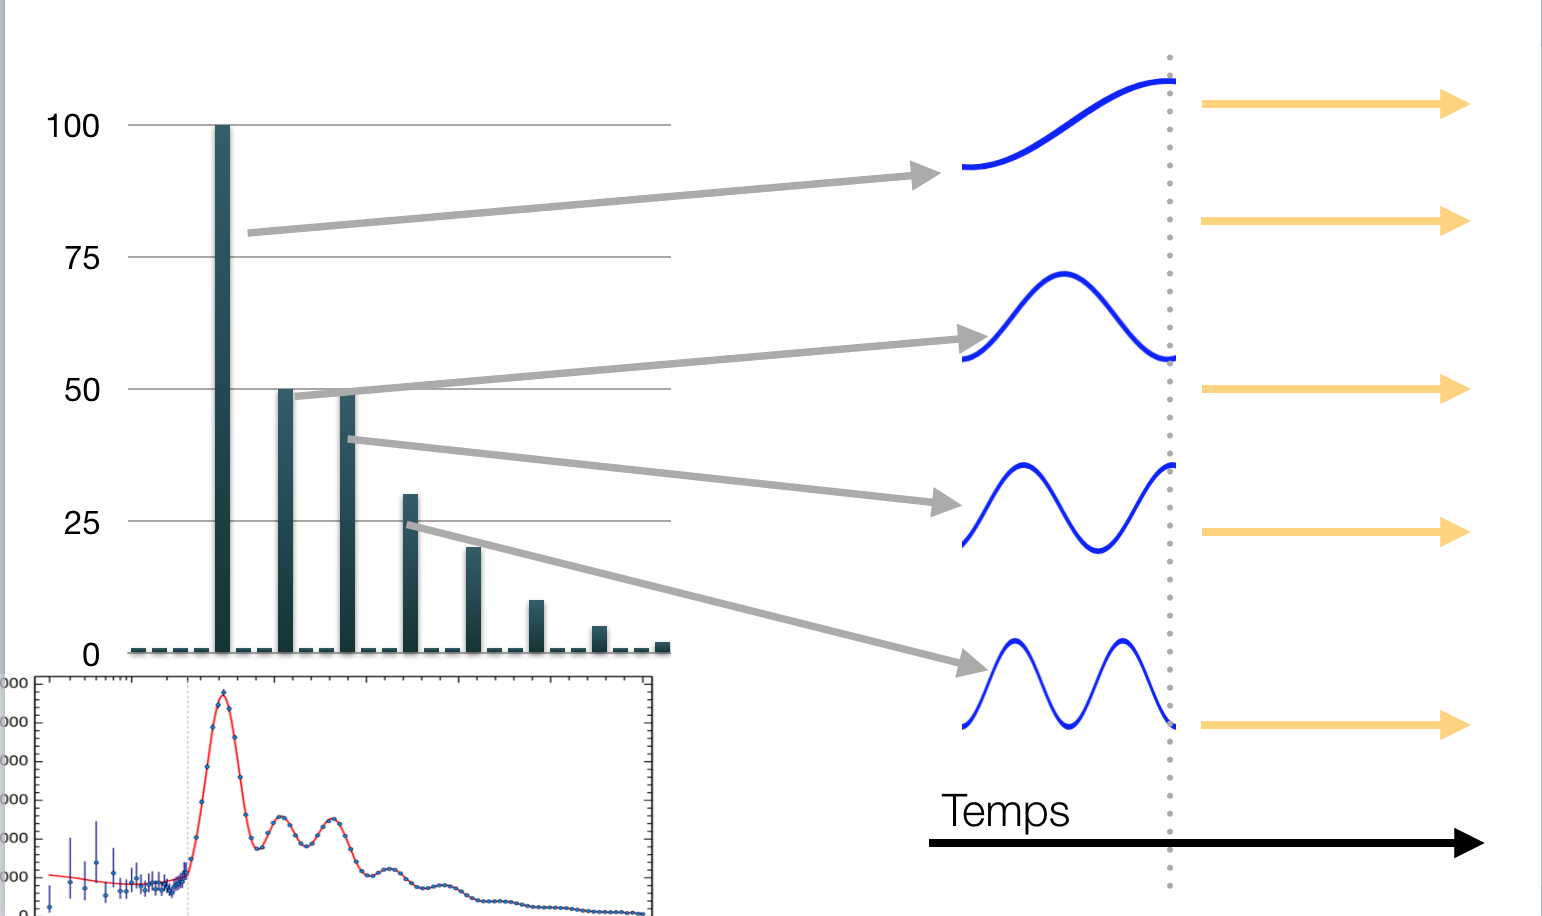
\includegraphics[height=12cm]{figs/bao2.png}
	\caption[Les pics accoustiques sont des extrema]{Les pics accoustiques du spectre de puissance du fond diffus cosmologique correspondent aux modes qui sont en extremum d'amplitude au moment de la recombinaison. Le premier pic correspond à une compression, le second une compression + une détente, le troisième une compression + une détente + une compression, etc.... Au premier ordre, nous voyons des harmoniques d'un même mode fondamental. }
	\label{f:bao2}
\end{figure}

\section{Croissance des perturbations : cas super-horizon}

Jusqu'à présent, nous nous sommes concentrés sur les petites échelles. Regardons à présente le comportement d'un mode de très grande taille, dont la longueur caractéristique est plus grande que \textit{l'horizon cosmologique} à l'instant considéré. Ces modes sont appelés super-horizon, tandis que les modes de petite taille précédemment étudié sont par analogie désignés comme étant sub-horizon.

\newthought{L'horizon}\index{horizon} désigne la plus grande échelle sur laquelle un phénomène de propagation peut opérer. Sa valeur est simplement donnée par :
\begin{equation}
L_H=\frac{c}{H}
\end{equation}
où $H^{-1}$ apparaît comme une mesure de l'âge de l'Univers à un instant donné. L'horizon est donc le produit de la plus grande vitesse par la plus grande durée. Son expression comobile présente une évolution temporelle qui dépend de la période de domination. Durant la période dominée par le rayonnement on a comme horizon comobile:
\begin{equation}
\ell_{H,RD}=\frac{c}{aH}\sim a
\end{equation} 
et durant la période dominée par la matière:
\begin{equation}
\ell_{H,MD}\sim\sqrt{a}.
\end{equation}
Dans les 2 cas, l'horizon grandit avec le temps et un mode de taille comobile donnée va donc successivement être plus grand que l'horizon (super-horizon) puis plus petit (sub-horizon) : usuellement, on désigne cette transition par l'expression \textit{passer sous l'horizon}. Le cas super-horizon demande un traitement en relativité générale complet donnant l'équation de croissance des structures suivantes:
\begin{equation}
\ddot \delta_k + 2H \dot \delta_k = \frac{3}{2}H^2(1+w)(1+3w)\delta_k
\end{equation}
où $w=0$ durant l'époque MD et $w=1/3$ durant l'époque RD \sidenote{pour ces échelles plus grandes que l'horizon, la pression ne peut jouer un role significatif: baryons et matière noire ont le même comportement}. 

Cette équation est similaire à celle obtenue dans le cas sub-horizon. Pour l'époque de domination de la matière on retrouve le même taux de croissance que celui obtenu pour la matière noire :
\begin{equation}
\delta_{k,MD}\sim t^{2/3}\sim a(t),
\end{equation}
tandis que durant l'époque de domination du rayonnement on obtient:
\begin{equation}
\delta_{k,RD}\sim t \sim a(t)^2.
\end{equation}


\section{Croissance des perturbations : synthèse et spectre de puissance}

La synthèse des résultats précédents pour le cas de la matière noire est présenté dans la figure \ref{f:perturb}. On constate qu'une petite perturbation peut voir son histoire de croissance gelée si elle passe sous l'horizon durant l'époque dominée par le rayonnement. A l'inverse un mode de grande longueur d'onde devra attendre la période dominée par la matière pour changer de régime et ne connaîtra pas la phase de non-croissance qu'auront connu les plus petites structures.

\begin{figure}[htbp]
	\centering
		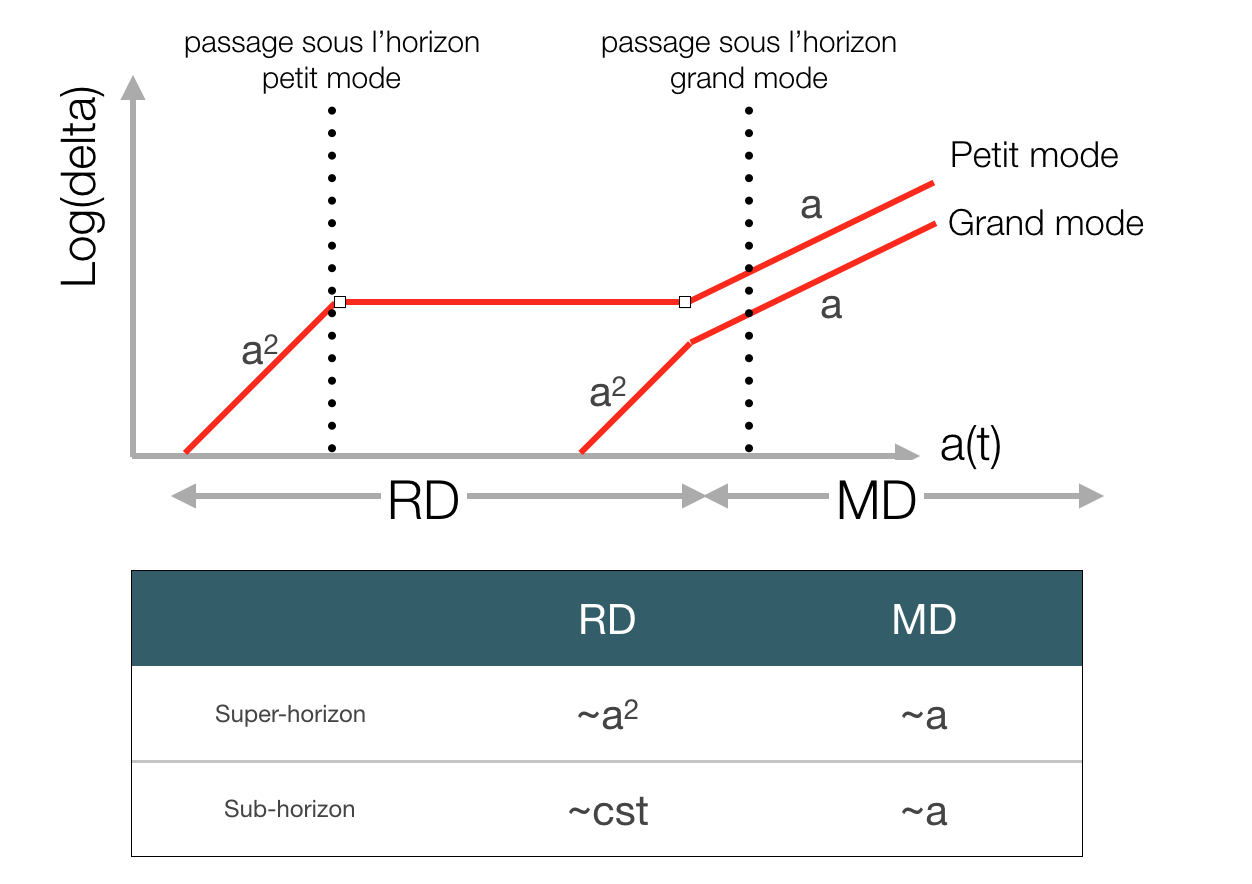
\includegraphics[height=8cm]{figs/perturb.png}
		\caption[Synthèse de la croissance des perturbations]{Synthèse de la croissance des perturbations. Un petit mode possède une taille caractéristique suffisemment petite pour passer sous l'horizon durant l'époque dominée par le rayonnement.}
	\label{f:perturb}
\end{figure}

Grâce à cette synthèse on peut prédire l'amplitude d'un mode au moment de la recombinaison $\delta_f$ en fonction de son amplitude $\delta_i$ bien avant l'équivalence matière-rayonnement. Considérons d'abord le cas d'un grand mode, sans période de gel de croissance, son amplitude au moment de l'équivalence est donné par:
\begin{equation}
\delta_e=\frac{a_e^2}{a_i^2}\delta_i.
\end{equation}
Son amplitude finale est alors donnée par :
\begin{equation}
\delta_f=\frac{a_f}{a_e}\delta_e=\frac{a_f a_e}{a_i^2}\delta_i.
\end{equation}
La chose importante est l'indépendance du facteur reliant l'amplitude initiale et finale vis à vis de la taille du mode : tous les modes vont croître dans les même proportions entre les instants $i$ et $f$. 

Pour les petits modes la situation est différente. L'amplitude au passage sous l'horizon est donnée par
\begin{equation}
\delta_L=\frac{a_L^2}{a_i^2}\delta_i.
\end{equation}
où $a_L$ est l'instant de passage sous l'horizon. L'amplitude au moment de l'équivalence est identique car la croissance est gelée et l'amplitude finale est alors donnée par:
\begin{equation}
\delta_f=\frac{a_f}{a_e}\delta_e=\frac{a_f}{a_e}\delta_L=\frac{a_L^2 a_f}{a_i^2 a_e}\delta_i.
\end{equation}
Ici le facteur de lien dépend de $a_L$ et donc de la taille du mode considéré. En effet cet instant est déterminé par $\lambda = \ell_{H,RD} \sim a_L$ donc 
\begin{equation}
\delta_f \sim \frac{1}{k^2} \delta_i.
\end{equation}
On a une coupure d'autant plus forte que la fréquence du mode est élevée, d'autant plus forte que la taille du mode considéré est petite.

\newthought{Pour le spectre de puissance}\index{spectre de Puissance}, les conséquences sont simples. Pour les $k$ suffisamment faibles on a 
\begin{equation}
P_f(k)\sim\delta_k^2 \sim P_i(k),
\end{equation}
par contre pour les hautes fréquences le spectre de puissance est filtré suivant la relation:
\begin{equation}
P_f(k)\sim \frac{1}{k^4} P_i(k)
\end{equation}
Comme le spectre de puissance primordial est en loi de puissance tel que \sidenote{on parle de spectre invariant d'échelle, comme prédit par exemple par l'inflation}:
\begin{equation}
P_i(k)\sim k
\end{equation}
on obtient un spectre caractéristique aux hautes fréquences en 
\begin{equation}
P_f(k)\sim\frac{1}{k^3}.
\end{equation}
Le spectre de puissance résultant possède donc 2 régimes caractéristiques, l'un aux grandes échelles en $P(k)\sim k$ et l'autre aux petites échelles en $P(k)\sim k^{-3}$. La transition entre les deux correspond à l'échelle qui passe sous l'horizon exactement au moment de l'équivalence (cf. Fig \ref{f:pk}).

\begin{figure}[htbp]
	\centering
		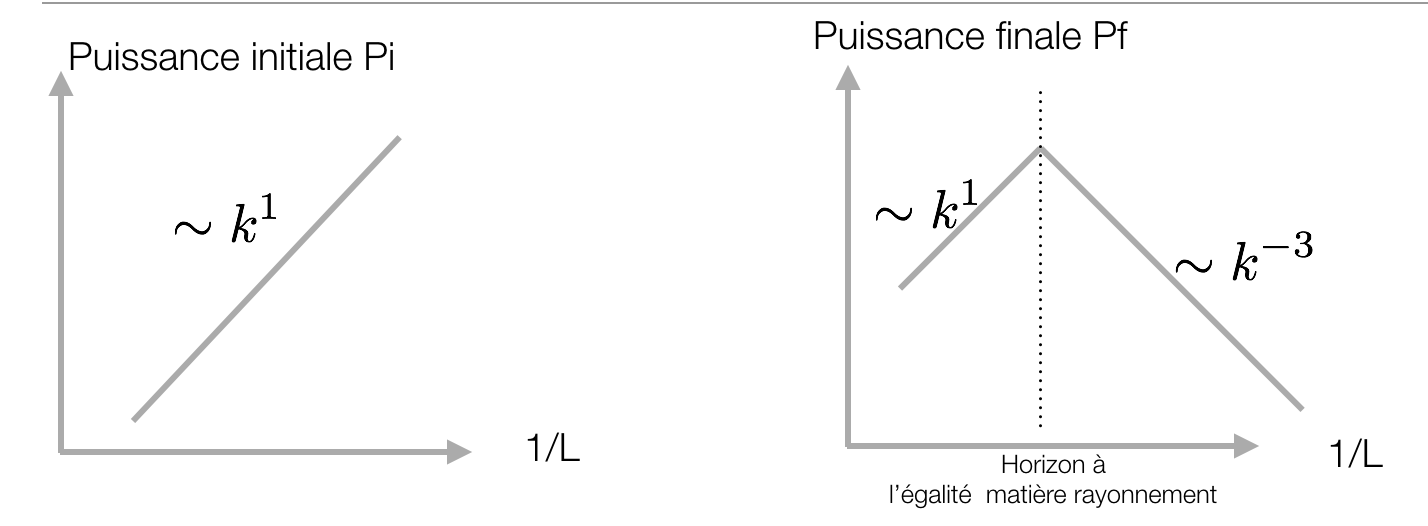
\includegraphics[height=8cm]{figs/pk.png}
		\caption[Schématique du filtrage du spectre de puissance des fluctuations initiales.]{Schématique du filtrage du spectre de puissance des fluctuations initiales. Le spectre primordial est invariant d'échelle en $P(k)\sim k$ et le gel de la croissance des fluctuations sous l'horizon durant l'époque de domination du rayonnement produit un filtrage au hautes fréquences qui produit une pente caractéristique en $P(k)\sim k^{-3}$.}
	\label{f:pk}
\end{figure}

\newthought{Pour résumer}, le spectre de puissance de la matière est une version filtrée du spectre de puissance primordial. Ce filtre opère sur les échelles suffisamment petites pour passer dans l'Horizon cosmologique tôt dans l'histoire de l'Univers, durant l'époque dominée par le rayonnement. Les échelles plus grandes ne permettant pas ce passage fréquence ont crû de façon indifférenciée et ont donc conservé les caractéristiques du spectre primordial. L'ensemble des prédictions développées dans ce chapitre, et notamment la mise en place du spectre de puissance $P(k)$ est fermement confirmée par de multiples observations (voir Fig. \ref{f:pktegmark})~: c'est un des grands succès du modèle $\Lambda$CDM aux grandes échelles.

\begin{figure}[htbp]
	\centering
		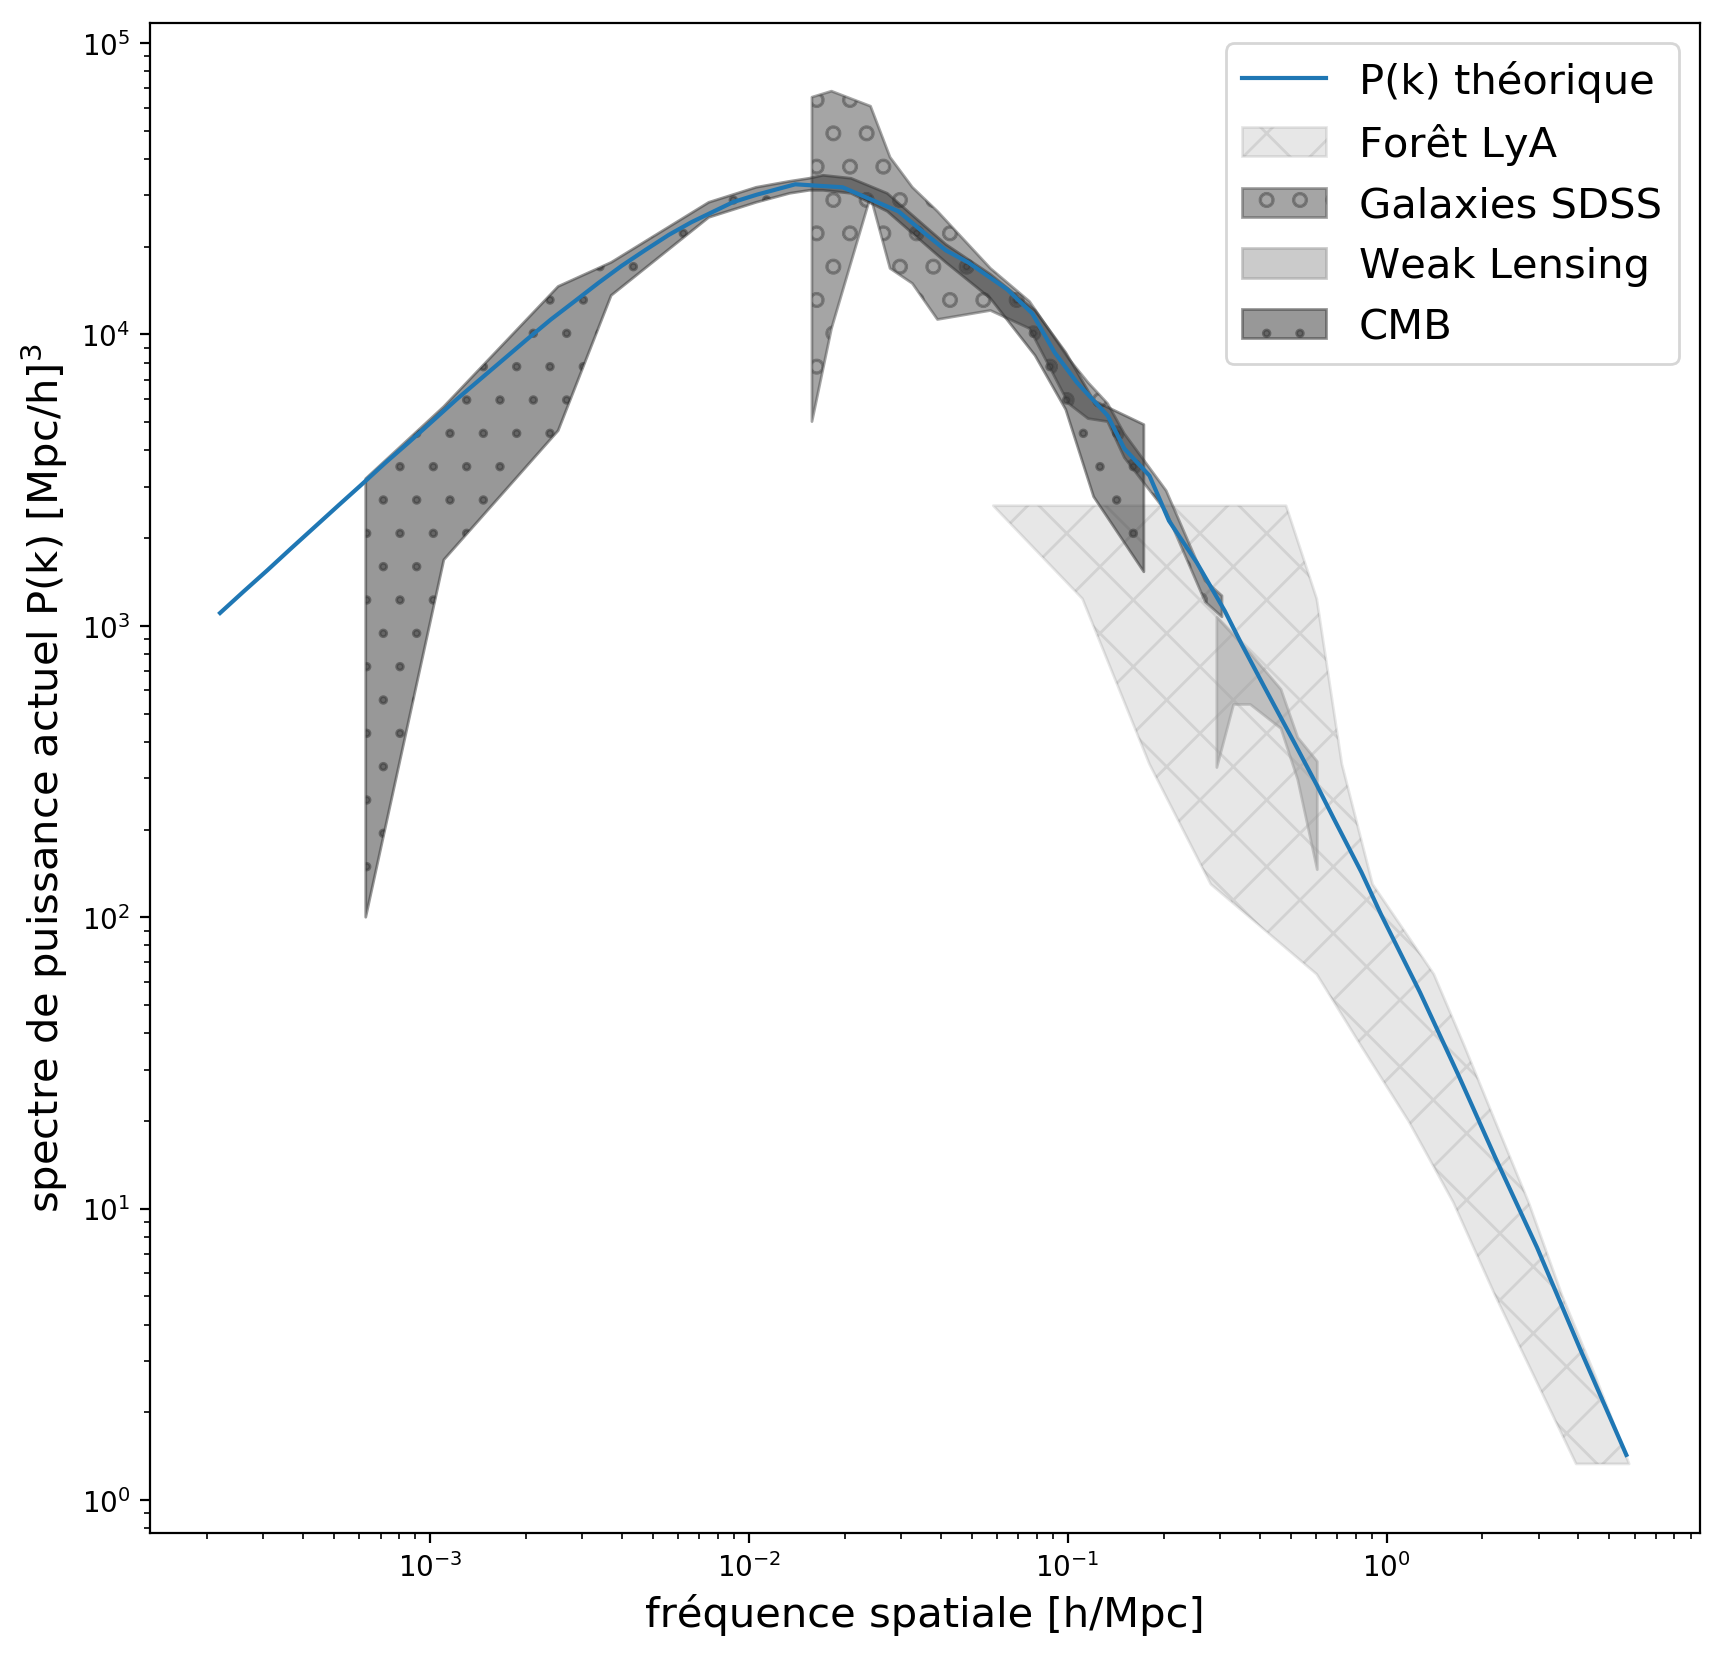
\includegraphics[height=12cm]{figs/pstegmark.png}
		\caption[Le spectre de puissance observé]{Le spectre de puissance $P(k)$ $\Lambda CDM$ théorique est représenté ici avec une compilation des estimations observationnelles issues de différentes sondes~: lensing, relevés de galaxies, CMB, comptage d'amas, Forêt Lyman-$\alpha$. On note l'excellent accord en théorie et prédiction.  Figure extraite de Tegmark et al. 2003. }
	\label{f:pktegmark}
\end{figure}


\newthought{Les oscillations baryoniques}\index{BAO}, mentionnées dans le cas de la matière avec pression et vues dans le CMB, se manifestent également dans le spectre de puissance de la matière totale. Ces ondes sonores se propageant dans le gaz vont légèrement modifier la structure globale de la matière : même si les baryons ne représentent qu'une faible fraction\sidenote{$\frac{\Omega_b}{\Omega_m}\sim0.15$} de la masse totale, cette fraction est non nulle et joue sur la dynamique globale à l'oeuvre. Ces oscillations se manifestent à nouveau comme des modes légèrement privilégiés dans le spectre de puissance $P(k)$. Par ailleurs, ces modes privilégiés vont persister dans la distribution de matière bien au delà de la recombinaison, jusqu'à nos jours. Par exemple, le spectre de puissance de la distribution actuelle des galaxies\sidenote{mesurée à z=0 dans des grands relevés de millions de galaxies comme le Sloane Digital Sky Survey (SDSS)}  présente des modes privilégiés aux fréquences attendues (voir Fig. \ref{f:percival}). De même, la distribution du gaz diffus intergalactique\index{IGM} à z=2\sidenote{sondée dans les spectres de Quasars distant} manifeste ces mêmes modes privilégiés. Ces ondes de pression primordiales, ont laissé leur empreinte dans toutes les structures qui ont émergé tout au long de l'histoire de l'Univers.

\begin{figure}[htbp]
	\centering
		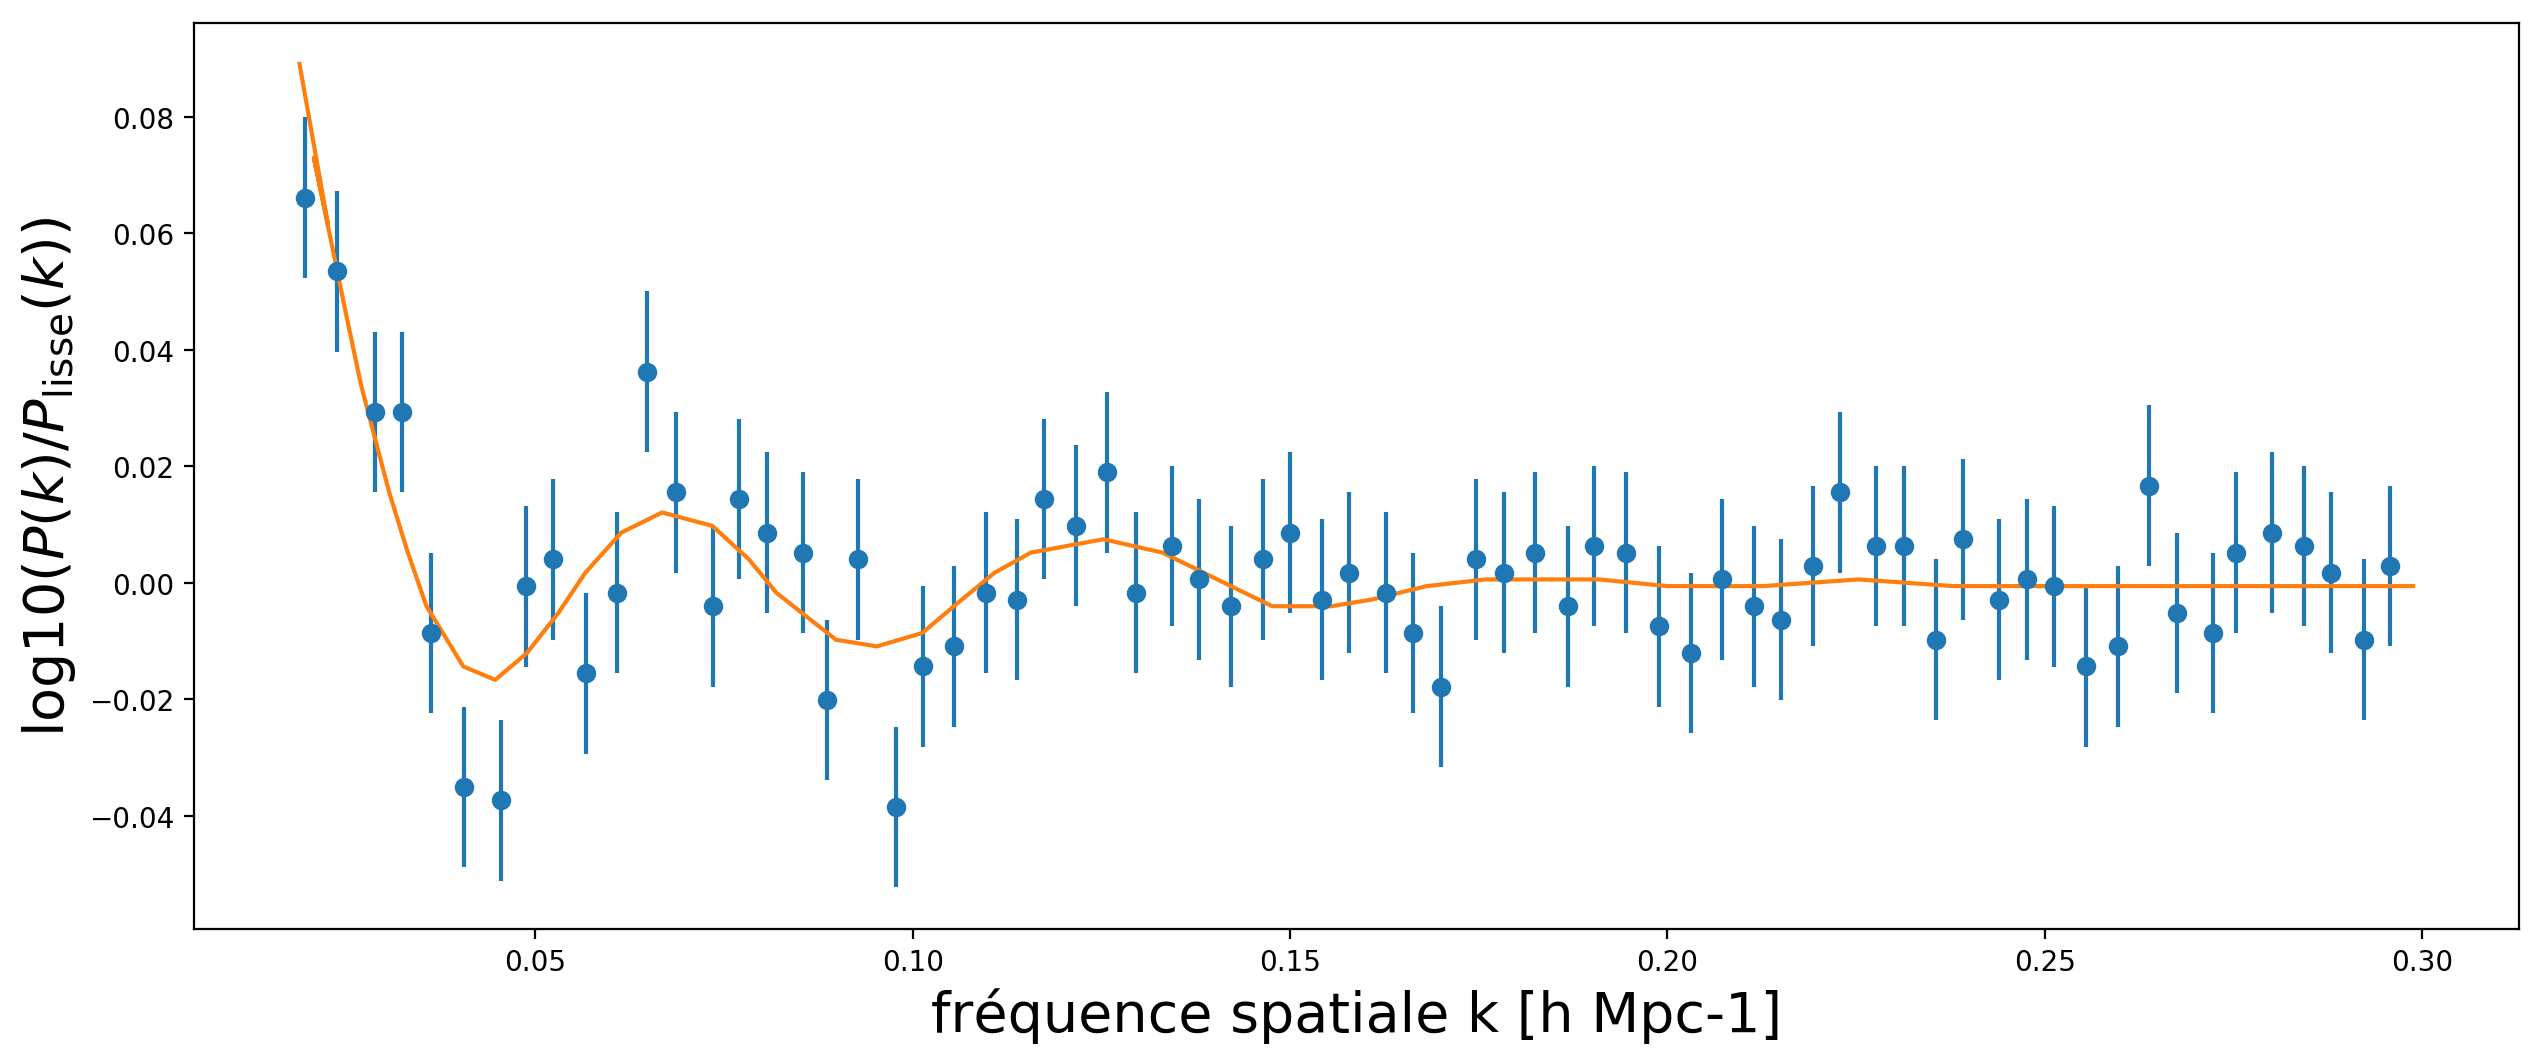
\includegraphics[height=12cm]{figs/percival.png}
		\caption[Les BAOs dans les relevés de galaxies]{Détection des BAOs dans le spectre de puissance du grand relevé de galaxies SDSS. Les courbes représentées sont le rapport du spectre mesuré dans les données sur le spectre lissé, sans BAO, pour 3 échantillons de galaxies différents. Les BAOs sont très clairement apparent (points) aux positions prédites par la théorie (lignes). Figure extraite de Percival et al. 2007.}
	\label{f:percival}
\end{figure}

\section{Et après ?}

Une fois le mécanisme d'instabilité déclenché, tous les modes vont parvenir à des régimes de surdensité qui vont au delà du régime linéaire et qui sortent du cadre dans lequel nous nous sommes placés. Dans certains cas académiques, le régime non linéaire peut-être abordé analytiquement mais en toute généralité il requiert l'utilisation de simulations numériques. La culmination de ce régime non linéaire est la création de structure denses, dominées par les baryons et au sein duquel se forment les sources de rayonnement : ce sont les galaxies qui nous entourent. L'apparition de ces objets est donc conditionnée par un contexte cosmologique et par extension il n'est pas illogique d'affirmer que l'étude de la formation des galaxies est une extension naturelle de la cosmologie. Toutefois, des phénomènes astrophysiques commencent à rentrer en jeu aux échelles considérées : thermodynamique du gaz, processus physico-chimique de refroidissement, champ magnétique, formation et rétroaction stellaire, production et impact des éléments plus lourds que l'hélium, etc.... Chacun de ces phénomènes est un objet d'étude à part entière et chacun de ces phénomènes est compris de façon toute relative. On en décrira quelques-uns ci-dessous, mais de façon générale on peut aisément avancer qu'aujourd'hui l'extension de la théorie cosmologique à celle de la formation des galaxies présente des défis majeurs. Ces défis, à l'heure où ces lignes sont écrites ne sont pas résolus.

\chapter{Formation des 'petites' structures}

\section{Au-delà du régime linéaire : le modèle d'effondrement sphérique}

\newthought{Une surdensité de matière} va nécessairement sortir du régime des faibles valeurs au bout d'un certain temps : le mécanisme d'instabilité gravitationnelle va condenser les structures vers des grandes densités et le jeu d'équations linéarisées utilisé ci-dessus n'est plus valable. Nous allons ici développer un modèle simple de surdensité qui permet de suivre l'évolution d'une telle structure en effondrement \index{effondrement sphérique}. Le destin d'une telle structure est de finir en halo de matière à l'équilibre, dont on exposera aussi les propriétés de base. A des fins de simplification, nous allons par la suite nous limiter au cas d'un Univers rempli uniquement de matière noire, non-collisionnelle, avec $\Omega_m=1$. Comme vu précédemment, cet Univers de Einstein-de Sitter\index{Einstein- de Sitter} est régi par une expansion en :
\begin{equation}
a(t) \sim t^{2/3}.
\end{equation}

Considérons une surdensité, sphérique de rayon $r$, baignant dans un Univers de densité $\bar \rho$. A l'intérieur de cette surdensité, la densité est initialement légèrement plus grande que celle du fond avec $\rho = (1+\delta) \bar \rho$ et uniforme à l'intérieur de ce rayon \sidenote{On parle aussi de modèle 'chapeau haut-de-forme' à cause du profil de densité en créneau associé }.  Ce modèle ressemble grandement au modèle de cosmologie newtonienne \index{cosmologie newtonienne} abordé en début d'ouvrage : dans ce modèle de cosmologie et pour la surdensité qui nous intéresse, sa dynamique est régie uniquement par la matière qui se trouve à l'intérieur et la couche la plus externe de la surdensité suit le principe fondamental de la dynamique :
\begin{equation}
\ddot r = -\frac{GM(<r)}{r^2}.
\end{equation}
Rappelons que $r(t)=a(t)r_0$ et dans le cas où cette couche est en expansion infinie \sidenote{ avec $\dot a >0$}, on peut facilement intégrer l'équation différentielle précédente pour obtenir :
\begin{equation}
r(t)=\left(\frac{9GM(<r)}{2}\right)^{1/3} t^{2/3},
\end{equation} 
avec une dépendance temporelle en $t^{2/3}$ conforme au modèle Einstein - de Sitter. Toutefois, cette dépendance ne peut représenter l'effondrement d'une structure, puisqu'on attend d'elle que son rayon diminue au delà d'un certain temps\sidenote{donc l'hypothèse $\dot a >0$ ne tient plus et nous empêche d'intégrer simplement l'équation différentielle}.

\newthought{La bon point de départ} est l'équation de conservation de l'énergie spécifique de la couche externe de notre structure :
\begin{equation}
E=\frac{\dot r^2}{2}-\frac{GM}{r}
\end{equation}
où $M=M(<r)$ désigne la masse à l'intérieur de la couche la plus externe. Rappelons que dans ce type de modèle les couches ne se croisent pas \sidenote{comme indiqué par $r(t)=a(t)r_0$ : une couche externe reste toujours une couche externe} et cette masse interne $M$ reste constante. Enfin, notre structure est vouée à s'effondrer, son énergie mécanique totale est donc négative, $E<0$. Dans ce type de situation, on peut montrer que la solution $r(t)$ s'exprime sous forme \textit{paramétrique} (voir aussi la figure \ref{f:rtparam}):
\begin{eqnarray}
r(\theta)&=&A (1-\cos \theta)\\
t(\theta)&=&B (\theta-\sin \theta)
\end{eqnarray}
où $\theta$ est un paramètre tel que $\theta \in [0,2\pi]$. La vitesse de la couche peut également s'écrire sous forme paramétrique\sidenote{obtenue en dérivant l'équation sur le temps puis en l'injectant dans celle sur le rayon}:
\begin{equation}
v(\theta)=\dot r= \frac{A \sin \theta}{B(1-\cos \theta)}.
\end{equation}
Ici, $A$ et $B$ sont respectivement des rayons et temps caractéristiques du problème traité avec :
\begin{eqnarray}
A&=&\frac{GM}{2|E|}\\
B&=&\frac{GM}{(2|E|)^{3/2}}\\
A^3&=&GM B^2
\end{eqnarray}
où la dernière relation est similaire à la troisième loi de Kepler qui relie période et rayon des orbites autour d'un corps massif.


\begin{figure}[htbp]
	\centering
		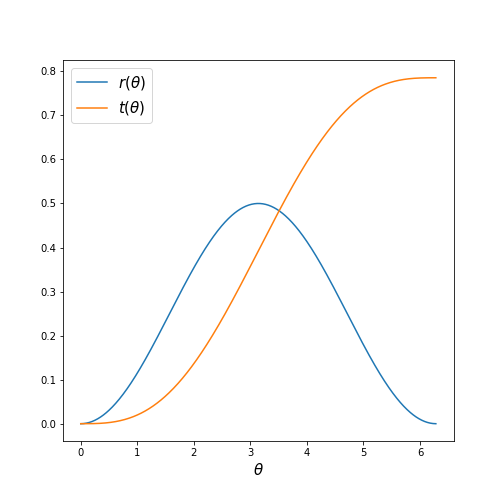
\includegraphics[height=10cm]{figs/rtparam.png}
		\caption[Les solutions paramétriques de l'effondrement sphérique]{Les solutions du modèle d'effondrement sphérique en fonction du paramètre $\theta$. Le temps $t$ est une fonction monotone de ce paramètre tandis que le rayon de la surdensité passe par un maximum, correspondant au découplage de la structure par rapport au fond cosmologique, avant de tendre vers 0 à la fin de l'effondrement.}
	\label{f:rtparam}
\end{figure}

Ces relations paramétriques permettent de caractériser les grandes étapes du processus d'effondrement. D'abord, on constate que l'évolution du rayon n'est pas monotone, celui-ci croît, atteint un maximum et décroit pour devenir nulle : notre surdensité évolue d'abord avec le fond, suivant l'expansion globale, puis elle atteint une extension maximale avant de se \textit{découpler} du flot global. La structure se réduit en taille avant d'atteindre une extension nulle et par conséquent sa densité devient infinie ! Cette évolution \sidenote{qui est la même que celle d'un Univers de densité supérieure à la densité critique} conduit naturellement à des régimes de densité non linéaires. Par simple inspection, on constate que le découplage, correspondant au maximum de $r$, opère pour $\theta=\pi$ et 
\begin{eqnarray}
r_d&=&2A\\
t_d&=&\pi B.
\end{eqnarray}
L'effondrement final correspond quant à lui à $\theta=2 \pi$ et 
\begin{eqnarray}
r_e&=&0\\
t_e&=&2\pi B.
\end{eqnarray}
Le temps nécessaire à l'effondrement \sidenote{on utilise aussi fréquemment les termes anglais de \textit{turn-around} pour le découplage et de \textit{collapse} pour l'effondrement} total de la structure est le double de celui nécessaire au découplage : $t_e=2 t_d$.

\newthought{La surdensité varie aussi de façon paramétrique}. La densité à l'intérieur de la structure est donnée par :
\begin{equation}
\rho = \frac{M}{4/3 \pi r^3}=\frac{3M}{4\pi A^3(1-\cos \theta)^3}, 
\end{equation}
tandis que la densité du fond, égale à la densité critique dans notre modèle est donnée par \sidenote{on rappelle que $H=\frac{\dot a}{a}$ et $a\sim t^{2/3}$ dans Einstein- de Sitter}:
\begin{equation}
\bar \rho =\frac{3H^2}{8\pi G}=\frac{1}{6\pi G t^2}=\frac{1}{B^2 6\pi G (\theta-\sin \theta)^2}.
\end{equation}
On obtient alors la formulation paramétrique de l'évolution de la surdensité :
\begin{equation}
\frac{\rho}{\bar \rho}=1+\delta=\frac{9}{2}\frac{(\theta - \sin \theta)^2}{(1-\cos \theta)^3}.
\label{e:dcoll}
\end{equation}
Bien sûr, cette équation ne rend pas compte des phases ultimes de l'effondrement : cet effondrement doit s'arrêter lorsqu'un équilibre est atteint après réorganisation de la matière et des vitesses. Les coquilles se croisent, la masse à l'intérieur de la coquille change et de l'énergie est échangée entre les couches.  

Toutefois, une bonne approximation du processus à l'oeuvre peut être obtenue en invoquant le théorème du Viriel. Une fois l'équilibre atteint, notre couche externe doit satisfaire
\begin{equation}
2 T +U = 0,
\end{equation}
où $T$ et $U$ désignent respectivement l'énergie cinétique et potentielle de notre couche externe après viriélisation. Comme par ailleurs l'énergie reste conservée, l'énergie totale en fin de viriélisation est donnée par:
\begin{equation}
E=\frac{U}{2}=-\frac{GM}{2r_v}
\end{equation}
où l'on considère que la masse interne n'a pas été modifiée significativement par la redistribution. A l'équilibre, l'énergie totale de la couche est complètement définie par son énergie potentielle : c'est également le cas lors du découplage, durant lequel l'énergie cinétique est nulle par définition\sidenote{en effet le découplage correspond au maximum d'extension de la surdensité avec $\dot r=0$ par définition}
\begin{equation}
E=-\frac{GM}{r_d}.
\end{equation}
Par conservation de l'énergie de la couche on obtient alors une relation entre le rayon de la couche externe à l'équilibre $r_v$ et celui lors du découplage $r_d$:
\begin{equation}
r_v\sim \frac{1}{2}r_d,
\end{equation}
le rayon de la structure se stabilise autour d'une valeur correspondant à la moitié du rayon lors du découplage. Ce rayon est aussi appelé \textit{rayon de viriel}, et est utilisé de façon générique pour désigner les bords 'externes' d'un halo de galaxie.

On peut également évaluer la valeur de la surdensité finale après la phase de viriélisation. On cherche à évaluer
\begin{equation}
1+\delta_\mathrm{v}=\frac{\rho(t_v)}{\bar \rho(t_v)},
\end{equation}
ce qui nécessite d'évaluer les deux densités $\rho$ et $\bar \rho$ post-viriélisation. La densité du fond est simple à obtenir, car la viriélisation opère au temps $t_v=t_e=2t_d=2\pi B$, on obtient donc:
\begin{equation}
\bar \rho(t_v) = \frac{1}{6\pi G t_v^2}=\frac{1}{4}\bar \rho (t_d).
\end{equation} 
De même, sachant que le rayon de viriel est la moitié du rayon de découplage, il existe une relation simple entre la densité à l'équilibre et celle lors du découplage:
\begin{equation}
\rho(t_v)=\frac{3 M}{4\pi r_v^3}=8 \rho(t_d)
\end{equation}
d'où la relation :
\begin{equation}
1+ \delta_v=\frac{8 \rho(t_d)}{\frac{1}{4}\bar \rho (t_d)}=32(1+\delta_d).
\end{equation}
Sachant que le découplage opère pour $\theta =\pi$, l'évaluation de l'équation \ref{e:dcoll} pour cette valeur donne $\delta_d\sim 5.55$ et une valeur de densité à l'équilibre 
\begin{equation}
1+\delta_v \sim 178.
\end{equation} 
En résumé, une structure qui s'effondre sous l'effet de l'instabilité gravitationnelle voit sa densité se stabiliser autour de 200 fois celle du fond. Pour cette raison, on désigne fréquemment le rayon de viriel $r_v$ sous le terme de $r_{200}$ et par exemple, c'est comme cela qu'on détermine l'extension d'un halo de galaxie dans une simulation numérique : son extension est choisie de telle façon à ce que la surdensité interne soit proche de 200.

\newthought{On peut également proposer une extrapolation linéaire} du calcul qui vient d'être réalisé. Il s'agit de calculer la surdensité au moment de l'effondrement mais telle qu'elle est prédite dans le régime linéaire. L'intérêt d'un tel calcul est qu'il permet de prédire simplement les régions qui vont s'effondrer sans avoir à réaliser un calcul non-linéaire complet : en se donnant un champ de densité, on peut prédire aisément sa croissance linéaire et désigner quelles régions vont s'effondrer et à quel instant. Si l'on reprend notre modèle paramétrique, le régime des faibles perturbations est celui qui opère au début, donc quand $\theta \ll 1$. Ce paramètre devient alors une simple fonction de $t$\sidenote{obtenu via un développement limité de $t(\theta)$} :
\begin{equation}
\theta \sim \left(\frac{6t}{B}\right)^{1/3}.
\end{equation}
De même dans ce régime et en utilisant les bons développements limités, l'équation \ref{e:dcoll} peut être réécrite :
\begin{equation}
1+\delta =\frac{9}{2}\frac{(\theta -\sin \theta)^2}{(1-\cos \theta)^3}\sim 1+\frac{3}{20} \theta^2.
\end{equation}
D'où l'expression de $\delta_l$ dans le régime linéaire en fonction du temps:
\begin{equation}
\delta_l=\frac{3}{20}\left(\frac{6t}{B}\right)^{2/3}=\frac{3}{20}(6\pi)^{2/3}\left(\frac{t}{t_d}\right)^{2/3}.
\end{equation}
On note d'ores et déjà que l'on retrouve la fameuse dépendance en $t^{2/3}$, propre aux modèles dominés par la matière. Au moment de l'effondrement, $t=t_e=t_v=2t_d$, ce qui donne $\delta_l=1.69$. Cette valeur revêt un caractère un peu 'magique' : si on évolue une champ de densité linéairement, les régions qui dépassent ce seuil vont s'effondrer. Ce type de raisonnement permet de prédire quelles régions vont former des structures et à quel instant : c'est ce qui permet par exemple de faire des prédictions analytiques sur la fonction de masse des halos de matière noire ou bien sur leur histoire de formation. Ce types de prédictions sont à la base de modèles \textit{analytiques} de formation des galaxies où la connaissance de l'histoire de formation de ces objets peut être utilisée pour prédire l'évolution des baryons en leur sein et les propriétés des galaxies qui s'y forment.

\begin{figure}[htbp]
	\centering
		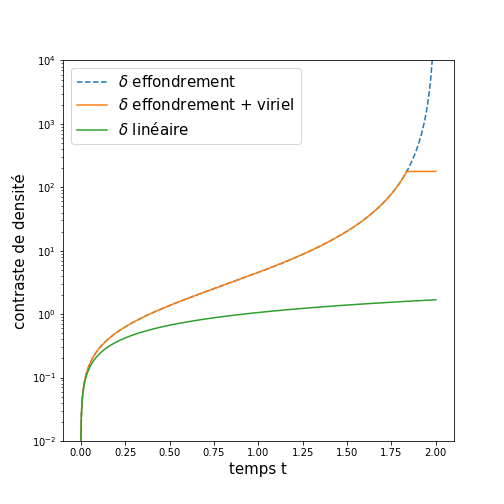
\includegraphics[height=10cm]{figs/delta_coll.png}
		\caption[Evolution temporelle du contraste de densité pour l'effondrement sphérique]{Les différentes solutions pour le contraste de densité $\delta=\rho/\bar \rho -1$ au cours du temps. On constate que le contraste non-linéaire évolue vers une singularité au moment de l'effondrement, la densité tend vers l'infini. Pratiquement, la surdensité va se stabiliser autour d'un contraste d'environ 200, correspondant à un état d'équilibre issu d'une redistribution de la matière et des vitesses appelée viriélisation. L'approximation linéaire suit la solution non-linéaire dans le régime des petits contrastes mais évolue plus lentement aux temps ultérieurs pour atteindre une valeur de 1.68 au moment où la structure devrait s'effondrer.}
	\label{f:dcoll}
\end{figure}


\section{Propriétés générique des halos post-effondrement}
Les structures effondrées étudiées dans la partie précédente sont de fait les halos de matière noire qui entourent les galaxies. Nous venons par exemple de prédire que la densité typique interne à ces objets doit être de l'ordre de 200 fois celle du fond, mais qu'en est-il du profil de densité de ces halos ? Les simulations cosmologiques montrent que le profil résultant de la viriélisation est de forme \textit{ universelle} et qu'une forme fonctionnelle simple permet d'ajuster le profil de la distribution de matière sur des grandes gammes de masses d'objet. La plus célèbre de ces formes fonctionnelles est le profil NFW \sidenote{du nom de ses découvreurs Navarro, Frenk et White} : 
\begin{equation}
\rho(r)=\frac{\rho_s}{(r/r_s)(1+r/r_s)^2}.
\end{equation}

\begin{figure}[htbp]
	\centering
		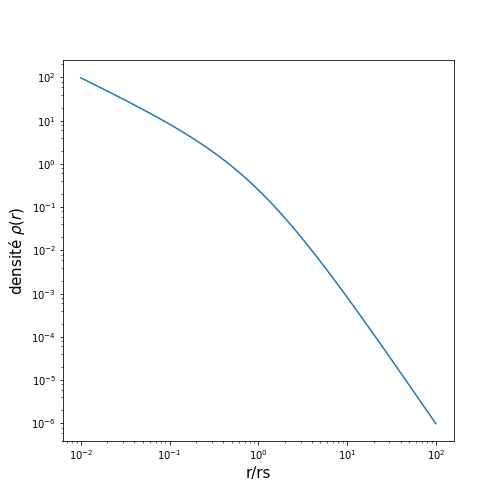
\includegraphics[height=9cm]{figs/nfw.png}
		\caption[Le profil de densité NFW]{Le profil de densité de NFW est le profil universel des halos de matière noire mesuré dans les simulations de formation des grandes structures. Ce profil se caractérise par le 'pic' en $r^{-1}$ au centre : ce type de distribution de matière n'est pas observé dans la cinématique des étoiles centrales des galaxies naines par exemple, posant difficulté aux prédictions des modèles de matière noire. L'injection répétée d'énergie dans le gaz central pourrait conduire à une redistribution de la matière dans ces régions, y compris dans la composante matière noire, pour 'aplatir' ce profil.}
	\label{f:nfw}
\end{figure}

Ce profil se comporte en $r^{-3}$ à grande distance et en $r^{-1}$ près du centre du halo et on qualifie ce profil de 'piqué'. Le rayon $r_s$ est le rayon de transition entre ces deux régimes de pentes à courte et grande distance. Les mêmes simulations montrent que le rapport entre ce rayon de transition et le rayon de viriel étudié précédemment, appelé aussi concentration, est de l'ordre de :
\begin{equation}
c=\frac{r_v}{r_s}\sim 10
\end{equation}
sachant que les petits halos sont plutôt plus concentrés que cette valeur et les plus massifs sont plutôt moins concentrés. Ce comportement piqué au centre n'est pas sans poser problèmes car les mesures de cinématiques au centre des galaxies naines semblent indiquer un profil de densité possédant plutôt un coeur plat \sidenote{avec des profils en $\rho \sim r^0$ }. Bien que cela soit encore un sujet de recherche actif, le consensus grandissant est que la physique baryonique, et notamment les processus d'injection d'énergie répétée dans le gaz par les générations successives de supernovae au centre des halos, conduirait à une redistribution des profils centraux de matière vers des profils à 'coeur' : c'est l'absence de prise en compte de ces effets dans les simulations qui conduirait à cette différence entre modèles et observations.

\newthought{Le gaz n'est pas en reste} dans le processus de viriélisation. Une fois l'équilibre atteint, le gaz va aussi s'organiser dans le potentiel gravitationnel du halo dominé par la matière noire. On peut par exemple lui assigner une température d'équilibre appelée aussi température de Viriel. Conformément au théorème du Viriel, l'équipartition entre énergie cinétique et potentielle des baryons peut s'écrire:
\begin{equation}
3\frac{M_gk_B T}{\mu m_p} - \alpha \frac{G M_v M_g}{r_v}=0.
\end{equation}
Ici $\mu mp$ désigne la masse typique d'une particule (atome d'hydrogène, hélium, électron), $M_g$ est la masse de gaz totale et $\alpha$ est un facteur de forme proche de l'unité dépendant du profil de masse du gaz. La température de viriel du gaz est donc une fonction simple de la masse et de la taille du halo : $T_v\sim M_v/r_v \sim V_v^2$ \sidenote{ici $V_v=\sqrt{GM_v/r_v}$ désigne la vitesse du Viriel, la vitesse circulaire au rayon de viriel, qui est une mesure de sa masse. }, et pour une masse de halo donné cela implique que si un processus quelconque (comme l'arrivée de rayonnement) chauffe le gaz au dessus de cette température, celui-ci ne peut rester à l'équilibre et éventuellement l'évaporer. Bien sûr la température du gaz à l'intérieur d'une vraie galaxie n'est pas constante et cette température de Viriel n'est qu'une estimation des régimes typiques des températures atteintes au sein des halos.

Toutefois, un gaz dispose d'un canal d'évacuation d'énergie interne inaccessible à la matière noire : les processus baryoniques régis par les interactions electro-magnétiques et la production de rayonnement qui peut emporter de l'énergie interne du gaz. On appelle ces processus des \textit{processus de refroidissement}, caractérisé par une fonction de refroidissement $\Lambda(x,T)$ qui dépend de la température du gaz $T$ et de sa fraction d'ionisation $x$\sidenote{$x=1$ désigne un gaz dont tous les atomes sont ionisés, $x=0$ où ils sont tous neutres} : la quantité d'énergie évacuée par le gaz, en $J/m^3/s$, est donnée par :
\begin{equation}
\Delta e_\mathrm{int}=n_H^2 \Lambda(x,T).
\end{equation}
Cette fonction de refroidissement dicte la quantité d'énergie évacuée à chaque instant par les processus atomiques d'excitation collisionnelle, d'ionisation, de recombinaison et de brehmstrahlung : tous ces processus dépendent du nombre d'atomes neutres et d'électrons disponibles, d'où la dépendance de la fonction de refroidissement en fraction d'ionisation. Ces processus de refroidissement produisent de la lumière, font diminuer l'énergie interne du gaz qui perd en support thermique et peut donc se contracter davantage : le gaz va devenir de plus en plus dense dans un halo de matière noire qui lui va rester à l'équilibre de viriel. La conséquence ultime de ce processus de condensation est la formation d'une galaxie et au sein de celle-ci la formation d'étoiles. Bien sûr, si le refroidissement n'est pas assez efficace, le gaz va retrouver son équilibre hydrostatique et l'effondrement du gaz n'aura pas lieu : la compétition entre ces deux effets s'évalue en comparant les temps de refroidissement et de rééquilibrage:
\begin{eqnarray}
t_\mathrm{ref}&\sim &\frac{n_H k_BT}{n_H^2\Lambda}\\
t_\mathrm{eq}&\sim &\frac{1}{\sqrt{G\rho}}.
\end{eqnarray}
On note que le temps d'équilibrage n'est rien d'autre que le temps d'effondrement dynamique, qui est le temps typique de réorganisation de la matière sous l'effet de la gravitation. Si $t_\mathrm{eq}\ll t_\mathrm{ref}$ le refroidissement n'est pas assez efficace, l'effondrement baryonique s'arrête. Dans le cas inverse, l'énergie peut être évacuée par rayonnement assez rapidement et la contraction est catastrophique pouvant in fine mener à la formation de galaxie et d'étoiles. On note que le refroidissement varie comme $\rho^{-1}$ tandis que l'équilibrage varie en $\rho^{-1/2}$ : plus le milieu est dense, plus le refroidissement est efficace par rapport à l'équilibrage et favorise ainsi l'effondrement. 

Quand on inspecte rapidement la fonction de refroidissement, on note celle-ci est maximale pour des températures comprises entre $10^4$ et $10^6$ degrés : en-dessous, les énergies ne sont pas suffisantes pour enclencher les processus atomiques, au dessus le gaz est trop ionisé, limitant les possibilités en termes de processus atomiques disponibles. Par conséquent, les halos trop légers, avec des températures de viriel trop faibles ($M_v<10^9 M_\odot$), ne peuvent refroidir efficacement. De même les objets très lourds ($M_v>10^{13} M_\odot$) présentent en principe les même limitations car possédant des températures caractéristiques trop élevées. En pratique toutefois, les plus gros objets disposent de sous régions denses qui refroidissent efficacement. De même, les plus petits objets bénéficie également de la possibilité de refroidir via les processus \textit{moléculaires} du $H_2$ notamment, qui étend les capacités de refroidissement à de plus faibles températures. De même la présence d'éléments plus lourds que l'hélium, désignés sous le terme de métaux, fournit de multiples transitions atomiques et multiplie les canaux d'évacuation de l'énergie : l'enrichissement du gaz par les générations successives d'étoiles favorise le refroidissement du gaz.

\begin{figure}[htbp]
	\centering
		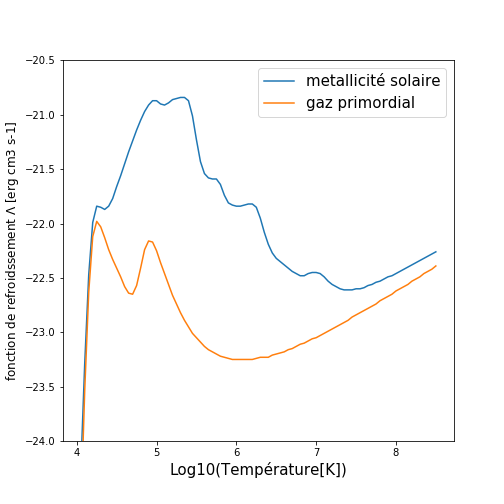
\includegraphics[height=10cm]{figs/cool.png}
		\caption[La fonction de refroidissement du gaz]{La fonction de refroidissement du gaz de Sutherland et Dopita, pour un gaz sans métaux, dit 'primordial' et un gaz avec une métallicité solaire. Dans les 2 cas, le refroidissement n'est efficace qu'au dessus de 10 000 K tandis que les hautes températures présente un comportement en $\sqrt{T}$ typique du Brehmstrahlung. Pour le gaz primordial on observe les 2 'bosses' caractéristiques des processus d'excitation collisionnelle de l'hydrogène et de l'hélium. Le gaz enrichi en métaux est globalement plus efficace car disposant des multiples canaux de refroidissement des éléments plus lourds que l'hélium. Les cas présentés ici suppose un équilibre d'ionisation.}
	\label{f:coolins}
\end{figure}


Pour finir, on a rapidement réalisé que lorsqu'il était actif, ce processus de refroidissement devenait trop efficace en particulier à grand redshift lorsque la matière était très dense, donnant des petites galaxies trop abondantes, un nombre trop important d'étoiles ou des galaxies de tailles trop faible, trop concentrées \sidenote{par exemple dans les travaux de White \& Rees à la fin des années 70 ou Navarro \& White dans les années 90s}. Il faut donc réinjecter de l'énergie dans le gaz pour qu'il arrête ce refroidissement catastrophique, via par exemple l'énergie injectée par les explosions d'étoiles en fin de vie ou par la présence d'un fond de rayonnement ultra-violet. On reviendra sur ces sujets dans la partie dédiée aux simulations numériques.